% @author Marcel Ruland (2018)
% !TEX encoding = UTF-8 Unicode
% !TEX TS-program = LuaLaTeX
\documentclass[aspectratio=169]{beamer}

\usetheme{Berlin}								% use Berlin theme
\setbeamercovered{transparent}					% set covered items to 85% alpha

\usepackage[english]{babel}						% English language support
\usepackage{ttjenevers}							% use TT Jenevers for rm
\usepackage{ttcommons}							% use TT Commons for sf
\setmonofont[Scale=MatchLowercase]{Envy Code R}	% use Envy Code R for tt
\usepackage{microtype}							% improved typography
\usepackage{natbib}								% bibliography
\bibliographystyle{newharvard}					% custom Harvard bibliography style

\newcommand{\sfmath}[1]{\(\mathsf{#1}\)}		% inline sf maths

\newcommand{\shorttitle}{Applying \textsc{fpm} to Multimodal Behaviour in Interaction}
\newcommand{\longtitle}{Applying Frequent Pattern Mining to \\ Multimodal Behaviour in Interaction}
\newcommand{\shortauthor}{K.~Rohlfing, {\addfontfeature{Style=Alternate}M.~Ruland}, S.~Henzgen}

\title[\shorttitle]{\longtitle}
\subtitle{Visualising Significant Patterns}
\institute{Paderborn University}
\author[\shortauthor]{Katharina Rohlfing \and {\addfontfeature{Style=Alternate}Marcel Ruland} \and Sascha Henzgen}% \\ \scriptsize{mruland@mail.upb.de}}%
\date[ECDA 2018]{July 8, 2018}

\begin{document}

\frame{\titlepage}
\frame{\frametitle{Outline}\tableofcontents}


\section{Preliminaries}
\frame{
	\frametitle{Basic Concepts}
	\begin{columns}
		\column{0.5\textwidth}
		\begin{itemize}
			\item turn
			\item turn-taking
			\item uni- vs multimodality
		\end{itemize}
		\column{0.5\textwidth}
		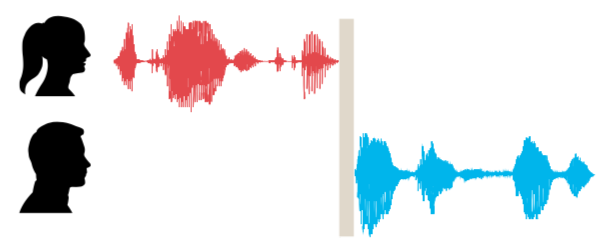
\includegraphics[width=0.5\textwidth]{../aux/img/dummy_basic_concepts.png}
	\end{columns}
}


\section{Method}
\frame{
	\frametitle{Video Material}
	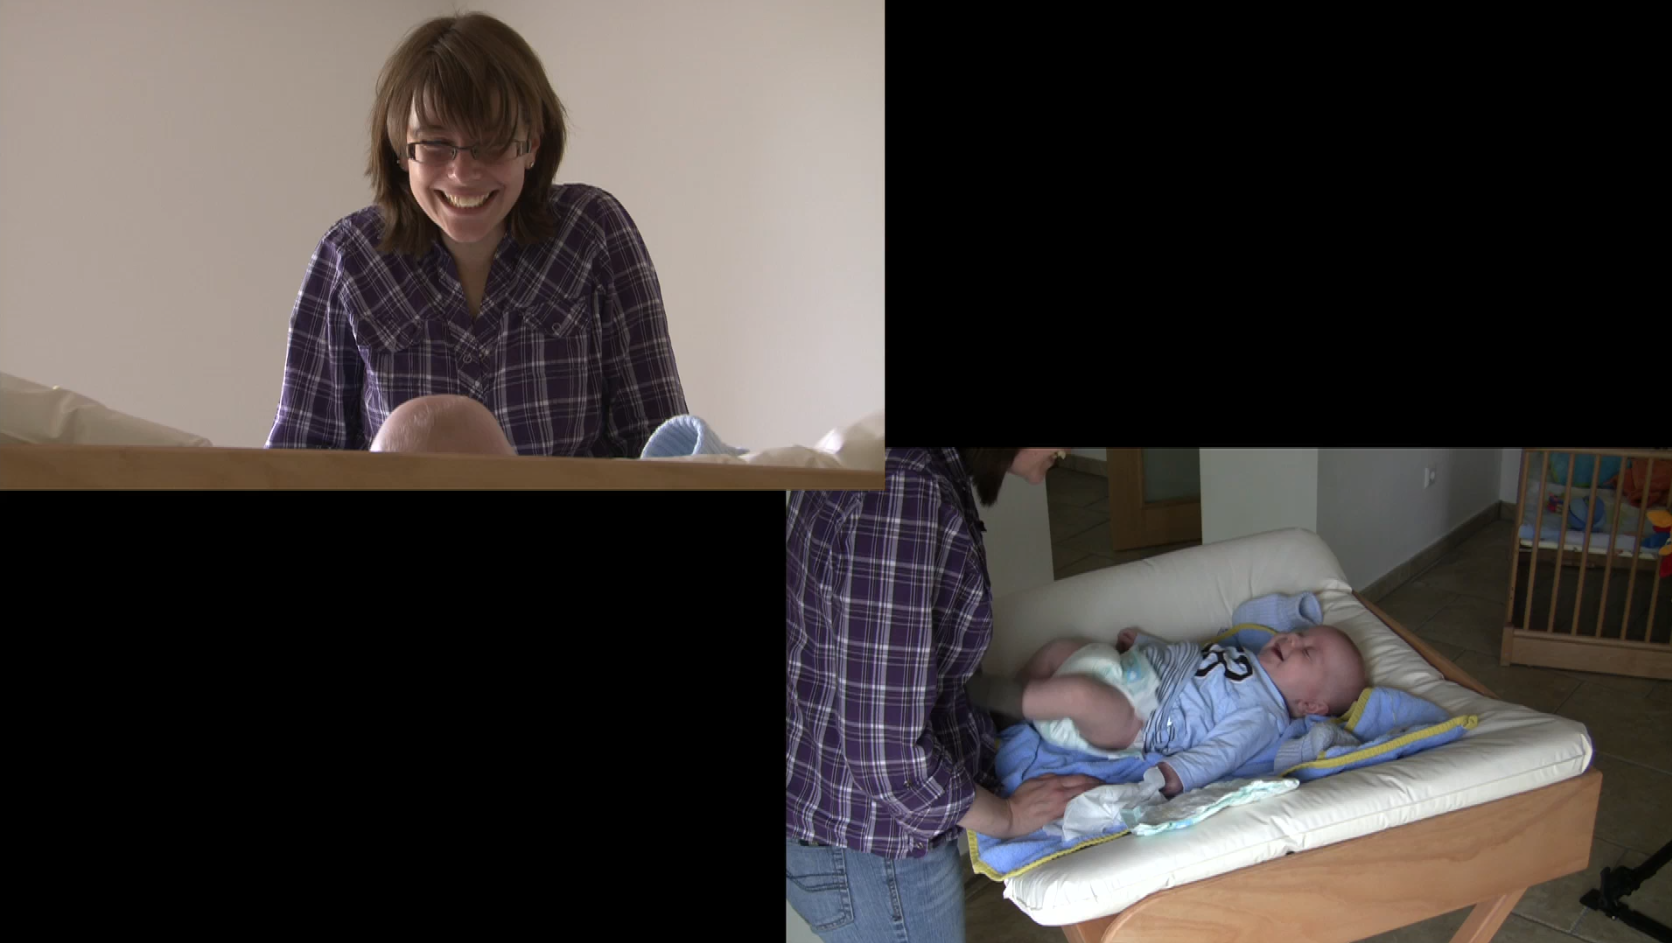
\includegraphics[height=0.8\textheight]{../aux/img/video_vp_08_raw.png}
}


\section[Significance]{Establishing Significance}
\frame{
	\frametitle{Significance -- Why would we care?}
	\begin{columns}
		\column{0.5\textwidth}
			Before:
			\begin{itemize}
				\item ``Why did you choose this rule?''
				\item ``Because it looked interesting to me.''
			\end{itemize}
		\column{0.5\textwidth}
			After:
			\begin{itemize}
				\item ``Why did you choose this rule?''
				\item ``Because it looked interesting to me. Also, the numbers support this claim''
			\end{itemize}
	\end{columns}
}


\frame{
	\frametitle{Bibliography}
	\bibliography{../bib/ba_bib}
}

\end{document}

%\frame{
%	\frametitle{Dummy}
%	\begin{columns}
%		\columns{0.5\textwidth}
%			left
%		\columns{0.5\textwidth}
%			right
%	\end{columns}
%}
